\documentclass[a4paper,12pt,oneside,final,titlepage]{article}
\usepackage[showframe=false, left=25mm,top=25mm,right=30mm,bottom=15mm]{geometry}
\usepackage{amsmath}
\usepackage{xeCJK}
\usepackage{changepage}
\usepackage{wrapfig}
\usepackage{fancyhdr}
\usepackage{tikz}
\usetikzlibrary{positioning,arrows,automata}
\pagestyle{fancy}


\rhead{119033910026-王巍}
\lhead{矩阵理论-作业-壹}
\author{王巍}
\title{计算理论第一次作业}
\date{119033910026}
\begin{document}
\maketitle
\noindent 1.
\begin{adjustwidth}{2em}{}
(1)\ M为00010时:
\begin{adjustwidth}{2em}{}
$q_{0}00010B\Rightarrow 0q_{0}010B\Rightarrow 00q_{0}010B\Rightarrow 000q_{0}10B\Rightarrow 0000q_{1}B\Rightarrow 00000q_{2}$
\end{adjustwidth}
(2)\ M为001000时:
\begin{adjustwidth}{2em}{}
$q_{0}001000B\Rightarrow 0q_{0}01000B\Rightarrow 00q_{0}1000B\Rightarrow 000q_{1}000B\Rightarrow 0000q_{1}00B\Rightarrow 00000q_{1}0B\Rightarrow 000000q_{1}B\Rightarrow 0000000q_{2}$
\end{adjustwidth}
(3)\ M为0010001时:
\begin{adjustwidth}{2em}{}
$q_{0}0010001B\Rightarrow 0q_{0}010001B\Rightarrow 00q_{0}10001B\Rightarrow 000q_{1}0001B\Rightarrow 0000q_{1}001B\Rightarrow 00000q_{1}01B\Rightarrow 000000q_{1}1B$ \\
没有对应转移函数,停机
\end{adjustwidth}
\end{adjustwidth}
2.
\begin{adjustwidth}{2em}{}
设图灵机$M = \{ Q, \Sigma, \Gamma, \delta, q_0, B, F \}$ \\
其中$Q = \{q_0, q_1, q_2 ,q_3\}, \ \Sigma = \{0, 1\},\ \Gamma = \{0, 1, B\},\ F = \{q_3\}$ \\
$\delta(q_0, 0) = (q_0, 0, R)\\ 
\delta(q_0, 1) = (q_1, 0, R)\\
\delta(q_1, 0) = (q_1, 0, R)\\
\delta(q_1, 1) = (q_2, 1, R)\\
\delta(q_2, 0) = (q_2, 0, R)\\
\delta(q_2, B) = (q_3, 0, R)$
\end{adjustwidth}
\begin{adjustwidth}{2em}{}
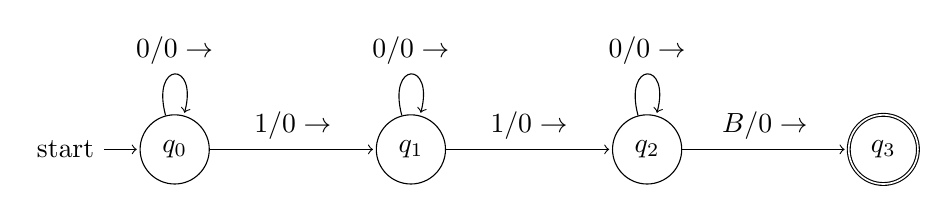
\begin{tikzpicture}[shorten >=1pt,node distance=3cm,on grid]
  \node[state,initial]   (q_0)                {$q_0$};
  \node[state]           (q_1) [right=of q_0] {$q_1$};
  \node[state] 			 (q_2) [right=of q_1] {$q_2$};
  \node[state,accepting] (q_3) [right=of q_2] {$q_3$};
  \path[->] (q_0) edge                node [above] {$1/0 \rightarrow$} (q_1)
                  edge [loop above]   node         {$0/0 \rightarrow$} ()
            (q_1) edge                node [above] {$1/0 \rightarrow$} (q_2)
            	  edge [loop above]	  node [above] {$0/0 \rightarrow$} ()
            (q_2) edge 				  node [above] {$B/0 \rightarrow$} (q_3)
            	  edge [loop above]	  node [above] {$0/0 \rightarrow$} ();
\end{tikzpicture}
\end{adjustwidth}
3.
\begin{adjustwidth}{2em}{}
(1)\ M为0011时:
\begin{adjustwidth}{2em}{}
$q_{0}0011B\Rightarrow Xq_{1}011B\Rightarrow X0q_{1}11B\Rightarrow Xq_{2}0Y1B\Rightarrow q_{2}X0Y1B\Rightarrow Xq_{0}0Y1B\Rightarrow XXq_{1}Y1B\Rightarrow XXYq_{1}1B\Rightarrow XXq_{2}YYB\Rightarrow Xq_{2}XYYB\Rightarrow XXq_{0}YYB\Rightarrow XXYq_{3}YB\Rightarrow XXYYq_{3}B\Rightarrow XXYYBq_{4}$
\end{adjustwidth}
(2)\ M为0101时:
\begin{adjustwidth}{2em}{}
$q_{0}0101B\Rightarrow Xq_{0}101B\Rightarrow q_{2}XY01B\Rightarrow Xq_{0}Y01B\Rightarrow XYq_{3}01B$\\
没有对应转移函数,停机
\end{adjustwidth}
(3)\ M为00111时:
\begin{adjustwidth}{2em}{}
$q_{0}00111B\Rightarrow Xq_{1}0111B\Rightarrow X0q_{1}111B\Rightarrow Xq_{2}0Y11B\Rightarrow q_{2}X0Y11B\Rightarrow Xq_{0}0Y11B\Rightarrow XXq_{1}Y11B\Rightarrow XXYq_{1}11B\Rightarrow XXq_{2}YY1B\Rightarrow Xq_{2}XYY1B\Rightarrow XXq_{0}YY1B\Rightarrow XXYq_{3}Y1B\Rightarrow XXYYq_{3}1B$\\
没有对应转移函数,停机
\end{adjustwidth}
\end{adjustwidth}
4.
\begin{adjustwidth}{2em}{}
(1)设图灵机$M = \{ Q, \Sigma, \Gamma, \delta, q_H, B, F \}$ 
\begin{adjustwidth}{2em}{}
其中$Q = \{q_H, q_e, q_{l1} ,q_{l2}, q_o, q_{else}, q_{acc}\}, \ \Sigma = \Gamma - \{B\},\ F = \{q_{acc}\}$, $\Gamma$为全部符号的集合(包括空白符号B) \\
令 $* = \Gamma,\quad \neg B = \Sigma$ ,则:\\ 
$\delta(q_H, *) = (q_e, H, R) \\
\delta(q_e, *) = (q_{l1}, e, R) \\
\delta(q_{l1}, *) = (q_{l2}, l, R) \\
\delta(q_{l2}, *) = (q_{o}, l, R) \\
\delta(q_o, *) = (q_{acc}, o, R) \\
\delta(q_{else}, \neg B) = (q_{else}, B, R) \\
\delta(q_{else}, B) = (q_{acc}, B, R)$
\end{adjustwidth}
\begin{adjustwidth}{2em}{}
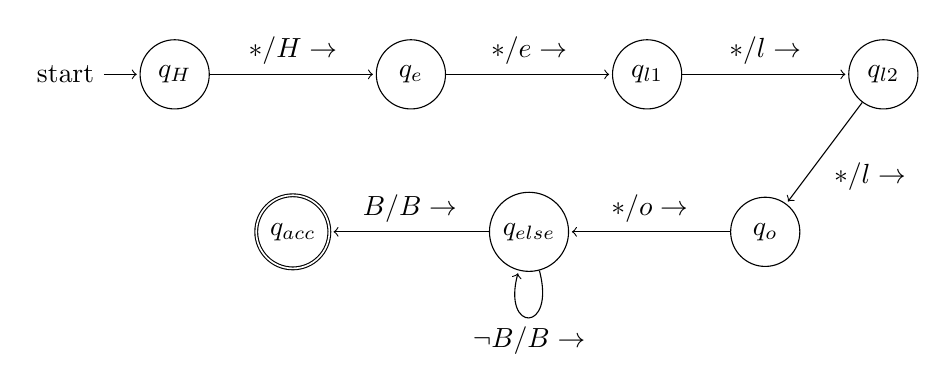
\begin{tikzpicture}[shorten >=1pt,node distance=3cm,on grid]
  \node[state,initial]   (q_H)                {$q_H$};
  \node[state]           (q_e) [right=of q_H] {$q_e$};
  \node[state] 			 (q_{l1}) [right=of q_e] {$q_{l1}$};
  \node[state] (q_{l2}) [right=of q_{l1}] {$q_{l2}$};
  \node[state] (q_o) [below left=2cm and 1.5cm of q_{l2}] {$q_o$};
  \node[state] (q_{else}) [left=of q_o] {$q_{else}$};
  \node[state,accepting] (q_{acc}) [left=of q_{else}] {$q_{acc}$};
  \path[->] (q_H)		edge	node 	[above] 		{$*/H \rightarrow$} (q_e)
  			(q_e)		edge	node 	[above] 		{$*/e \rightarrow$} (q_{l1})
  			(q_{l1})	edge	node 	[above] 		{$*/l \rightarrow$} (q_{l2})
  			(q_{l2})	edge	node 	[below right]			{$*/l \rightarrow$} (q_o)
  			(q_o)		edge	node 	[above] 		{$*/o \rightarrow$} (q_{else})
  			(q_{else})	edge	[loop below]	node 	[below] 	{$\neg B/B \rightarrow$} ()
  						edge 	node 	[above]			{$B/B \rightarrow$} (q_{acc});
\end{tikzpicture}
\end{adjustwidth}
(2)设图灵机$M = \{ Q, \Sigma, \Gamma, \delta, q_{Bye-B}, B_0, F \}$ 
\begin{adjustwidth}{2em}{}
其中$Q = \{q_{Bye-B}, q_{Bye-y}, q_{Bye-e}, q_{Hello-H},q_{Hello-e},q_{Hello-l1},q_{Hello-l2},q_{Hello-o}, q_{scan}, q_{acc}\}, \\ \Sigma = \Gamma - \{B_0\},\ F = \{q_{acc}\}$, $\Gamma$为全部符号的集合(包括空白符号$B_0$) \\
令 $* = \Gamma,\quad \neg B_0 = \Sigma $ ,则:\\ 
$\delta(q_{Bye-B}, B) = (q_{Bye-y}, B, R) \\
\delta(q_{Bye-y}, y) = (q_{Bye-e}, y, R) \\
\delta(q_{Bye-e}, e) = (q_{scan}, e, R) \\
\delta(q_{scan}, B_0) = (q_{Hello-H}, B_0, L) \\
\delta(q_{Hello-H}, \neg B_0) = (q_{Hello-H}, B_0, L) \\
\delta(q_{Hello-H}, B_0) = (q_{Hello-e}, H, R) \\
\delta(q_{Hello-e}, B_0) = (q_{Hello-l1}, e, R) \\
\delta(q_{Hello-l1}, B_0) = (q_{Hello-l2}, l, R) \\
\delta(q_{Hello-l2}, B_0) = (q_{Hello-o}, l, R) \\
\delta(q_{Hello-o}, B_0) = (q_{acc}, o, R) \\$
\end{adjustwidth}
\begin{adjustwidth}{2em}{}
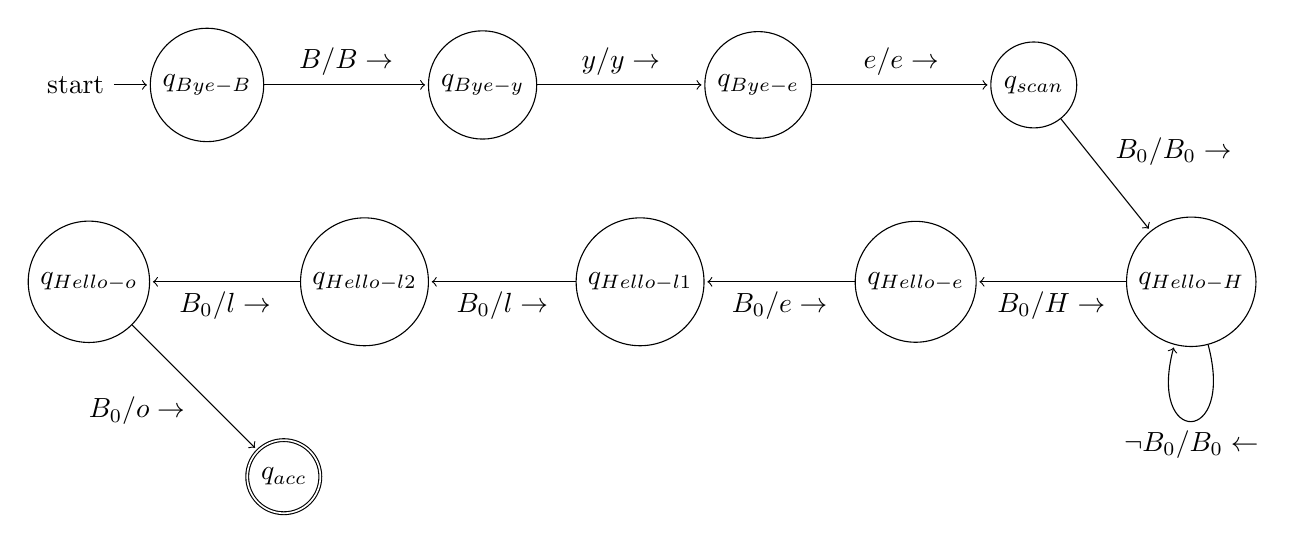
\begin{tikzpicture}[shorten >= 1pt, node distance=3.5cm, on grid]
\node[state, initial] 		(q_{Bye-B})								{$q_{Bye-B}$};
\node[state]				(q_{Bye-y}) [right=of q_{Bye-B}]		{$q_{Bye-y}$};
\node[state]				(q_{Bye-e})	[right=of q_{Bye-y}]		{$q_{Bye-e}$};
\node[state]				(q_{scan})	[right=of q_{Bye-e}]		{$q_{scan}$};
\node[state]				(q_{Hello-H})	[below right=2.5 cm and 2cm of q_{scan}]		{$q_{Hello-H}$};
\node[state]				(q_{Hello-e})	[left=of q_{Hello-H}]	{$q_{Hello-e}$};
\node[state]				(q_{Hello-l1})	[left=of q_{Hello-e}]	{$q_{Hello-l1}$};
\node[state]				(q_{Hello-l2})	[left=of q_{Hello-l1}]	{$q_{Hello-l2}$};
\node[state]				(q_{Hello-o})	[left=of q_{Hello-l2}]	{$q_{Hello-o}$};
\node[state, accepting]		(q_{acc})	[below right=of q_{Hello-o}]	{$q_{acc}$};
\path[->] 	(q_{Bye-B})		edge	node 	[above] 		{$B/B \rightarrow$} (q_{Bye-y})
			(q_{Bye-y})		edge	node 	[above] 		{$y/y \rightarrow$} (q_{Bye-e})
			(q_{Bye-e})		edge	node 	[above] 		{$e/e \rightarrow$} (q_{scan})
			(q_{scan})		edge	node 	[above right] 		{$B_0/B_0 \rightarrow$} (q_{Hello-H})
			(q_{Hello-H})	edge [loop below]	node 	[below]	{$\neg B_0/B_0 \leftarrow$} ()
							edge 	node 	[below]			{$B_0/H \rightarrow$} (q_{Hello-e})
			(q_{Hello-e})	edge	node 	[below] 		{$B_0/e \rightarrow$} (q_{Hello-l1})
			(q_{Hello-l1})	edge	node 	[below] 		{$B_0/l \rightarrow$} (q_{Hello-l2})
			(q_{Hello-l2})	edge	node 	[below] 		{$B_0/l \rightarrow$} (q_{Hello-o})
			(q_{Hello-o})	edge	node 	[below left] 	{$B_0/o \rightarrow$} (q_{acc});
\end{tikzpicture}
\end{adjustwidth}
\end{adjustwidth}
5.
\begin{adjustwidth}{2em}{}
(1)
\begin{adjustwidth}{2em}{}
设图灵机$M = \{ Q, \Sigma, \Gamma, \delta, q_0, B, F \}$ \\
其中$Q = \{q_0, q_1, q_2, q_3,q_4,q_5,q_6\},\ \Sigma = \{0, 1, 2\},\ \Gamma = \{0, 1, 2, X, Y, Z, B\},\ F = \{q_6\}$\\
$
\delta(q_0, 0) = (q_1, X, R) \\
\delta(q_0, Y) = (q_4, Y, R) \\
\delta(q_1, 0) = (q_1, 0, R) \\
\delta(q_1, Y) = (q_1, Y, R) \\
\delta(q_1, 1) = (q_2, Y, R) \\
\delta(q_2, 1) = (q_2, 1, R) \\
\delta(q_2, Z) = (q_2, Z, R) \\
\delta(q_2, 2) = (q_3, Z, L) \\
\delta(q_3, 0) = (q_3, 0, L) \\
\delta(q_3, 1) = (q_3, 1, L) \\
\delta(q_3, Y) = (q_3, Y, L) \\
\delta(q_3, Z) = (q_3, Z, L) \\
\delta(q_3, X) = (q_0, X, R) \\
\delta(q_4, Y) = (q_4, Y, R) \\
\delta(q_4, Z) = (q_5, Z, R) \\
\delta(q_5, Z) = (q_5, Z, R) \\
\delta(q_5, B) = (q_6, B, R)
$
\end{adjustwidth}
\begin{adjustwidth}{2em}{}
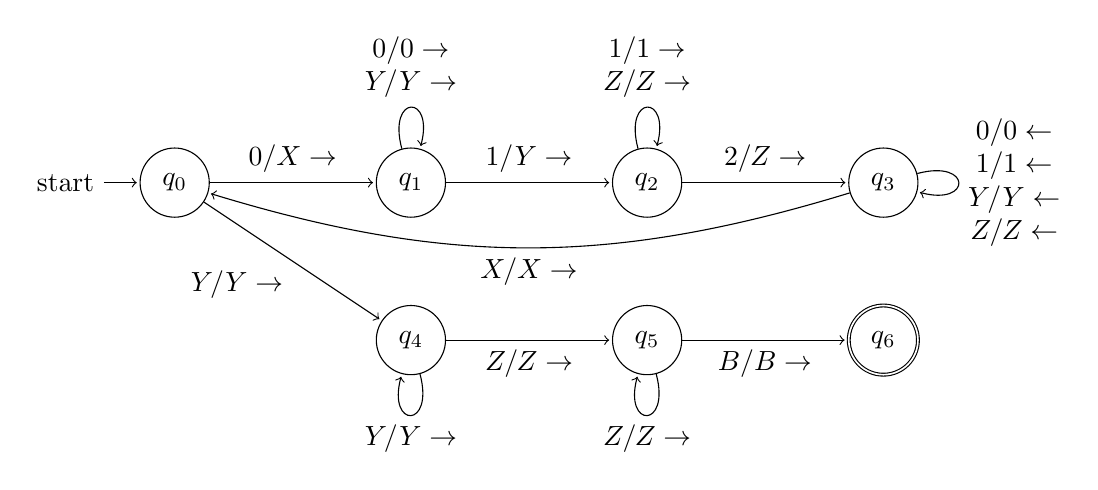
\begin{tikzpicture}[shorten >= 1pt, node distance=3cm, on grid]
\node[state, initial] 		(q_0)								{$q_0$};
\node[state]				(q_1) 	[right=of q_0]		{$q_1$};
\node[state]				(q_2)	[right=of q_1]		{$q_2$};
\node[state]				(q_3)	[right=of q_2]		{$q_3$};
\node[state]				(q_4)	[below=2cm of q_1]	{$q_4$};
\node[state]				(q_5)	[right=of q_4]		{$q_5$};
\node[state, accepting]		(q_6)	[right=of q_5]		{$q_6$};
\path[->]	(q_0)		edge		node 		[above]			{$0/X \rightarrow$} (q_1)
						edge		node 		[below left]			{$Y/Y \rightarrow$}	(q_4)
			(q_1)		edge	[loop above]	node 	[align=center]	{$0/0 \rightarrow$\\$Y/Y \rightarrow$} ()
						edge		node 		[above]			{$1/Y \rightarrow$} (q_2)
			(q_2)		edge	[loop above]	node 	[align=center]	{$1/1 \rightarrow$\\$Z/Z \rightarrow$} ()
						edge		node 		[above]			{$2/Z \rightarrow$} (q_3)
			(q_3)		edge	[loop right]	node 	[align=center]	{$0/0 \leftarrow$\\$1/1 \leftarrow$\\$Y/Y \leftarrow$\\$Z/Z \leftarrow$} ()
						edge 	[bend left=17]	node 	[below]	{$X/X \rightarrow$} (q_0)
			(q_4)		edge	[loop below]	node 			{$Y/Y \rightarrow$} ()
						edge		node 		[below]			{$Z/Z \rightarrow$} (q_5)
			(q_5)		edge	[loop below]	node 	[below]	{$Z/Z \rightarrow$} ()
						edge 		node 		[below] 		{$B/B \rightarrow$} (q_6);
\end{tikzpicture}
\end{adjustwidth}
(2)
\begin{adjustwidth}{2em}{}
假设$L = \{0^n1^n2^n|n\geq 1\}$是上下文无关语言,则L满足泵引理 \\
取$z = 0^N1^N2^N\in L,\ z = uvwxy$\\
由泵引理,存在这样的$z$使得$|vwx|\leq N$,则$vwx$最多包含两种字符,即$01\ \text{或}\ 12$,分类讨论:\\
i.若$vwx$仅包含0或1或2,以0为例,有:
\begin{adjustwidth}{2em}{}
取$uv^2wx^2y$,显然0的个数多于1和2,$uv^2wx^2y\notin L$,矛盾
\end{adjustwidth}
ii.若$vwx$仅包含$01\ \text{或}\ 12$,以$01$为例,有:
\begin{adjustwidth}{2em}{}
不妨设$v = 0^t1^s, w = 1^l$,取$uv^2wx^2y$ \\
$uv^2wx^2y = 0^{N+t}1^sw1^{1l}y$,显然0的数量多于2,$uv^2wx^2y\notin L$,矛盾 \\
当$x = 0^t1^s$时,同理有0和1的数量都多于2,矛盾
\end{adjustwidth}
故$L = \{0^n1^n2^n|n\geq 1\}$不是上下文无关语言
\end{adjustwidth}
\end{adjustwidth}
6.
\begin{adjustwidth}{2em}{}
思路:
\begin{adjustwidth}{2em}{}
向右扫描遇到第一个字符a,向左回到B,向右找到1-a并改成X,向左回到B,向右扫描遇到第一个非X的字符b,改成X,向左回到起点,向右找字符1 - b改成X $\cdots$ 
\end{adjustwidth}
解:
\begin{adjustwidth}{2em}{}
设图灵机$M = \{ Q, \Sigma, \Gamma, \delta, q_{found}, B, F \}$ \\ 
其中$Q = \{q_{found}, q_{search-0}, q_{search-1}, q_{back}, q_{acc}\}, \ \Sigma = \{0, 1\},\ \Gamma = \{0, 1, X, B\},\ F = \{q_{acc}\}$\\
$\delta(q_{found}, 0) = (q_{search-1}, X, L) \\
\delta(q_{found}, 1) = (q_{search-0}, X, L) \\
\delta(q_{found}, X) = (q_{found}, X, R) \\
\delta(q_{found}, B) = (q_{acc}, B, R) \\
\delta(q_{search-0}, 0) = (q_{back}, X, L) \\
\delta(q_{search-0}, 1) = (q_{search-0}, 1, R) \\
\delta(q_{search-0}, X) = (q_{search-0}, X, R) \\
\delta(q_{search-1}, 1) = (q_{back}, X, L) \\
\delta(q_{search-1}, 0) = (q_{search-1}, 0, R) \\
\delta(q_{search-1}, X) = (q_{search-1}, X, R) \\
\delta(q_{back}, 0) = (q_{back}, 0, L) \\
\delta(q_{back}, 1) = (q_{back}, 1, L) \\
\delta(q_{back}, X) = (q_{back}, X, L) \\
\delta(q_{back}, B) = (q_{back}, q_{found}, R) 
$
\end{adjustwidth}
\begin{adjustwidth}{2em}{}
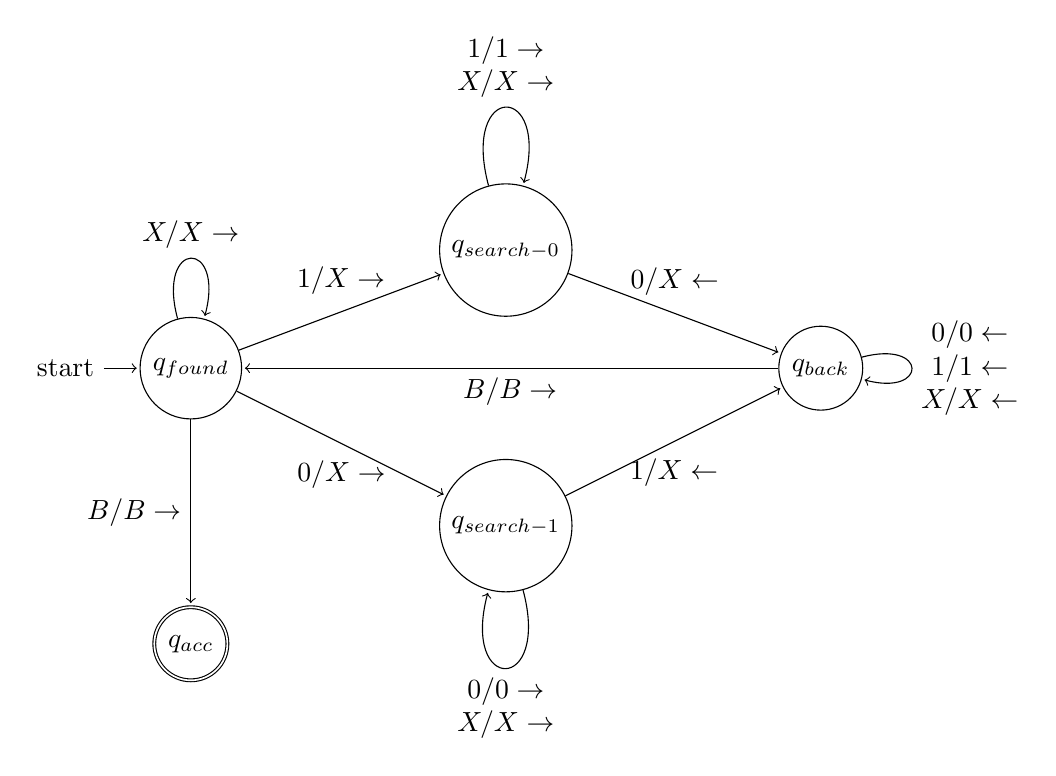
\begin{tikzpicture}[shorten >= 1pt, node distance=3.5cm, on grid]
\node[state, initial] 		(q_{found})									{$q_{found}$};
\node[state]				(q_{search-0}) [above right=1.5cm and 4cm of q_{found}]			{$q_{search-0}$};
\node[state]				(q_{search-1})	[below right=2cm and 4 cm of q_{found}]		{$q_{search-1}$};
\node[state]				(q_{back})	[above right=2cm and 4cm of q_{search-1}]	{$q_{back}$};
\node[state, accepting]		(q_{acc})	[below =of q_{found}]	{$q_{acc}$};
\path[->]	(q_{found})		edge	node 		[below=0.1cm]  	{$0/X \rightarrow$}	(q_{search-1})
							edge 	node 		[above=0.1cm]	 	{$1/X \rightarrow$} 	(q_{search-0})
							edge [loop above]		node 		[above]		{$X/X \rightarrow$}()
							edge 	node 		[left] 		{$B/B \rightarrow$} (q_{acc})
			(q_{search-0})	edge [loop above]	node 		[align=center] {$1/1 \rightarrow$ \\ $X/X \rightarrow$}()
							edge 	node 		[above=0.1cm]		{$0/X \leftarrow$} (q_{back})
			(q_{search-1})	edge [loop below]	node 		[align=center] {$0/0 \rightarrow$ \\ $X/X \rightarrow$}()
							edge 	node 		[below=0.1cm]		{$1/X \leftarrow$} (q_{back})
			(q_{back})		edge [loop right]	node 		[align=center] {$0/0 \leftarrow$ \\ $1/1 \leftarrow$\\$X/X \leftarrow$} ()
							edge 	node 		[below]		{$B/B \rightarrow$} (q_{found});
\end{tikzpicture}
\end{adjustwidth}
\end{adjustwidth}
7.
\begin{adjustwidth}{2em}{}
思路:
\begin{adjustwidth}{2em}{}
扫描遇到第一个字符,用状态记录这个字符,找到字符串末尾,和记录对比,相同则改为B,走到最左,进行下一轮$\cdots$
\end{adjustwidth}
解:
\begin{adjustwidth}{2em}{}
设图灵机$M = \{ Q, \Sigma, \Gamma, \delta, q_{found}, B, F \}$ \\ 
其中$Q = \{q_s, q_{found-0}, q_{found-1}, q_{search-0}, q_{search-1}, q_{back}, q_{acc}\}, \ \Sigma = \{0, 1\},\ \Gamma = \{0, 1, B\},\ F = \{q_{acc}\}$\\
$\delta(q_{s}, 0) = (q_{found-0}, B, R) \\
\delta(q_{s}, 1) = (q_{found-1}, B, R) \\
\delta(q_{s}, B) = (q_{acc}, B, R) \\
\delta(q_{found-0}, 0) = (q_{found-0}, 0, R) \\
\delta(q_{found-0}, 1) = (q_{found-0}, 1, R) \\
\delta(q_{found-0}, B) = (q_{search-0}, B, L) \\
\delta(q_{found-1}, 0) = (q_{found-1}, 0, R) \\
\delta(q_{found-1}, 1) = (q_{found-1}, 1, R) \\
\delta(q_{found-1}, B) = (q_{search-1}, B, L) \\
\delta(q_{search-0}, 0) = (q_{back}, B, L) \\
\delta(q_{search-1}, 1) = (q_{back}, B, L) \\
\delta(q_{back}, 0) = (q_{back}, 0, L) \\
\delta(q_{back}, 1) = (q_{back}, 1, L) \\
\delta(q_{back}, B) = (q_{s}, B, R)
$
\end{adjustwidth}
\begin{adjustwidth}{2em}{}
\begin{tikzpicture}[shorten >= 1pt, node distance=3.5cm, on grid]
\node[state, initial] 		(q_s)										{$q_s$};
\node[state]				(q_{found-0})  	[above right=1.5cm and 3cm of q_{found}]	{$q_{found-0}$};
\node[state]				(q_{found-1})	[below right=1.5cm and 3cm of q_{found}]		{$q_{found-1}$};
\node[state]				(q_{search-0}) 	[right=of q_{found-0}]		{$q_{search-0}$};
\node[state]				(q_{search-1})	[right=of q_{found-1}]		{$q_{search-1}$};
\node[state]				(q_{back})	[above right=1.5cm and 3cm of q_{search-1}]	{$q_{back}$};
\node[state, accepting]		(q_{acc})	[below =of q_s]	{$q_{acc}$};
\path[->] 	(q_s)			edge	node		[above=0.1cm]	{$0/B \rightarrow$}	(q_{found-0})
							edge	node		[below=0.1cm]	{$1/B \rightarrow$}	(q_{found-1})
							edge	node		[left]			{$B/B \rightarrow$}	(q_{acc})
			(q_{found-0})	edge	[loop above]	node 	[align=center]	{$0/0 \rightarrow$\\$1/1 \rightarrow$} ()
							edge	node 		[above]			{$B/B \leftarrow$}	(q_{search-0})
			(q_{found-1})	edge	[loop below]	node 	[align=center]	{$0/0 \rightarrow$\\$1/1 \rightarrow$} ()
							edge	node 		[below]			{$B/B \leftarrow$}	(q_{search-1})
			(q_{search-0})	edge	node 		[above right]	{$0/B \leftarrow$}	(q_{back})
			(q_{search-1})	edge	node 		[below right]	{$1/B \leftarrow$}	(q_{back})
			(q_{back})		edge	[loop right]	node 	[align=center]	{$0/0 \leftarrow$\\$1/1 \leftarrow$} ()
							edge	node 		[below]			{$B/B \rightarrow$} (q_s);

\end{tikzpicture}
\end{adjustwidth}
\end{adjustwidth}
\end{document}
